\startchapter{Background}
\label{chapter:background}

\section{IEEE 802.11ah Standrad}

 The IEEE 802.11ah standard is one of the recent standards by IEEE standard organization. This standard introduces many new concepts for the first time, including new designs for both the physical and MAC layers. The 802.11ah standard has been designed with three use cases in mind, smart sensors, back-haul aggregation and extended range hot-spot. In smart sensor use case, 802.11ah is designed to handle a very large number of nodes (up to 6000) connected to one access point. In the back-haul use case, an 802.11ah access point is designed to be used as an aggregator for wireless personal area network (WPAN) devices that use the IEEE 802.15.4.g standard. WPAN (802.15.4g) devices have a small transmission range and lower data rate, so in this case, 802.15.4g routers gather data from 802.15.4g devices and send them to a single 802.11ah aggregator. In the extended hot-spot use case, 802.11ah access points can be used as candidates for cellular offloading, specially in outdoor environment where other 802.11 standards suffer from their short transmission ranges.

\subsection{Physical Layer of IEEE 802.11ah}
In the Physical Layer (PHY), 802.11ah makes use of sub 1GHz license-exempt bands. This is the main physical layer difference between this standard and the previous 802.11 standards. Also, 802.11ah mostly focuses on small bandwidths and does not allow any channel with $>$20 MHz bands. The use of lower carrier frequency gives 802.11ah a much larger transmission range compared to other 802.11 standards as the path loss increases with regard to carrier frequency. In outdoor scenarios, using default transmission power (200mW), 1MHz channel and Modulation and Coding Scheme (MCS) 10, an 802.11ah device can achieve a range as high as 1 km \cite{khorov2015survey}. 

\subsection{Medium Access Control layer of IEEE 802.11ah}
 In the Medium Access Control (MAC) layer, 802.11ah introduces may new concepts from shortened frame formats to channel access and power management. In the main 802.11 standard, the number of nodes that can be connected to one access point is limited to 2007. IEEE 802.11ah extends this range to 8191 nodes to support the smart sensor use case. Also to better support dense network scenarios, 802.11ah shortens the length of frame headers, control frames such as ACKs and periodically transmitted frames such as beacon messages. The main change in 802.11ah which is also the focus of this thesis are the modifications in the channel access. 

 In order to handle the severe contentions between nodes in dense scenarios, 802.11ah divides all nodes connected the access point into different groups, and each group is given a specified time window called Restricted Access Window (RAW) to use the wireless channel while members of all other groups remain silent. This essentially divides the beacon period into multiple RAWs each dedicated to one group. It not only decreases the contention that one node experiences while using the wireless channel, but also lets nodes save power by going to sleep in the RAWs that do not belong to them. It is left to the access point to decide whether or not to allow nodes to cross the RAW boundary just to finish an ongoing transmission (Cross Slot Boundary). This channel access mechanism is called Group Synchronized Distributed Coordination Function (GS-DCF) which is to be used in 802.11ah instead of the traditional DCF.   

\section{The Hidden Terminal Problem}
\begin{figure} [th]
  \centering
  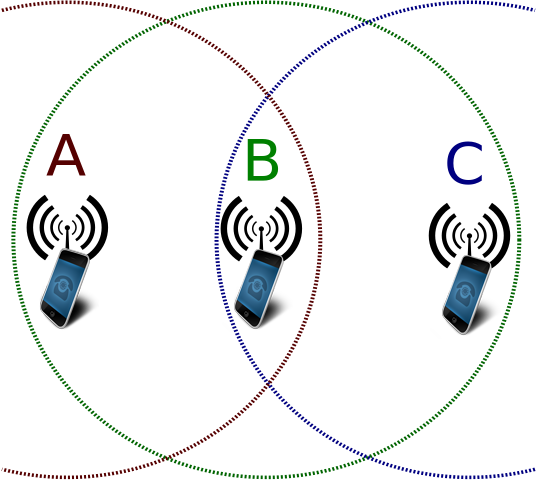
\includegraphics[width=.65\textwidth]{figures/hidden}
  \caption{A simple illustration of hidden terminal problem}
  \label{fig:hidden}
\end{figure}

The hidden terminal problem is a well-known issue in wireless communication networks. It usually happens when a node falls outside of the sensing area of another node but they are both trying to transmit simultaneously. Fig. \ref{fig:hidden} illustrates a general case for the hidden terminal problem. For example, if node A, first starts the transmission of a packet to node B and in the middle of their communication, node C also decides to transmit a packet to B or another node. According to the Carrier-Sense Multiple Access with Collision Avoidance (CSMA/CA) procedure, used in many wireless MAC protocols, it will first listen to the channel, and since it cannot sense the signal coming from A, it will find the channel idle and initiate its transmission which will result in a collision at B and loss of both packets from A and C. The uplink transmissions in Wireless LANs at the infrastructure mode, where several wireless nodes want to transmit to the access point, are vulnerable to this problem. 


The legacy solution for this problem is the use of Request To Send (RTS) and Clear To Send (CTS) messages. Using these messages, every node has to send an RTS packet to its receiver and wait until it gets a CTS packet before starting a transmission. Within the RTS and CTS packets, there is a Network Allocation Vector (NAV) which announce the anticipated channel occupation duration so any nodes receiving RTS or CTS should refrain from transmission during the time reserved according to NAV. In this way, although node C might not sense the RTS from node A, it will receive the CTS that B sends to A and know that the channel for B is going to be busy. The only chance of collision because of the hidden terminal then, is during the transmission of the RTS message. Since the RTS is a small control message, collision probability will be reduced significantly. 

Given the extended range of communication in the 802.11ah standard, the hidden terminal problem becomes even more serious, and the RTS/CTS solution may not be effective in dense networks when the number of nodes trying to transmit RTS simultaneously becomes large.



\section{Physical Layer Network Coding}

The concept of Network Coding is nothing new in the wireless domain. It relies on optimizing transmission of data by combining two or more messages in a network. Physical Layer Network Coding(PNC) is then a network coding happening at the physical layer.

We use a three node linear network example to illustrate this idea \cite{zhang2006hot}. In Fig. \ref{fig:justThreeNodes}, nodes $A$ and $B$ have packets to exchange and node $R$ can act as a relay.


\begin{figure} [th]
    \centering
    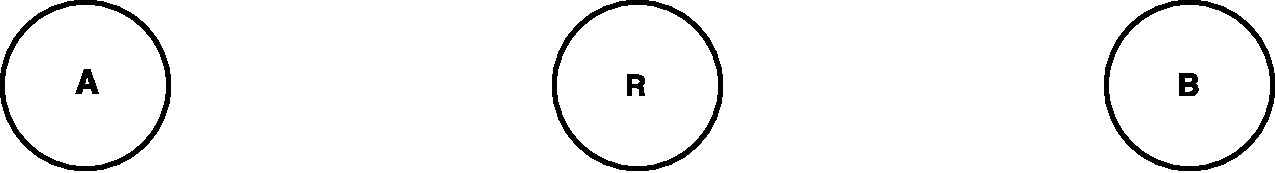
\includegraphics[width=0.8\textwidth]{figures/justThreeNodes.pdf}
    \caption{Simple three node linear network. Nodes $A$ and $B$ have packets to exchange and node $R$ acts as relay} \label{fig:justThreeNodes}
\end{figure}

Assuming that $A$ and $B$ are too far for a reliable transmission, there are different ways for this exchange of packets to happen, traditional relaying, straightforward network coding and physical layer network coding.

An exchange of packets between $A$ and $B$ where relay only works as a traditional decode and forward node takes four time slots as illustrated in Fig. \ref{fig:traditionalRelay}.  

\begin{figure} [th]
    \centering
    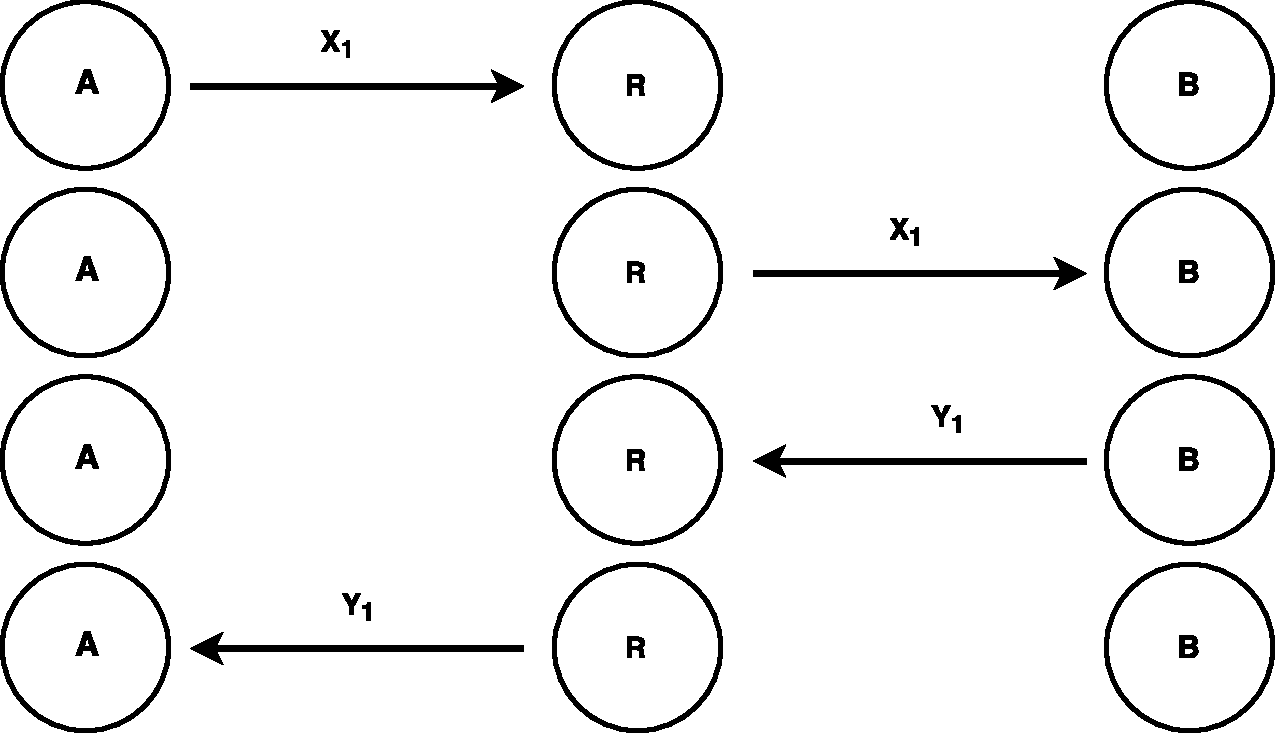
\includegraphics[width=0.8\textwidth]{figures/traditionalRelay.pdf}
    \caption{Traditional relaying. First, node $A$ transmits its packet to the relay, then the relay forwards $A$'s packet to $B$, then in time slot three, node B sends its packet to the relay, which is then forwarded to node $A$ in time slot four.} \label{fig:traditionalRelay}
\end{figure}

Using straightforward network coding, reduces the number of time slots required for that aforementioned exchanged to happen to three. Fig. \ref{fig:straightforwardNC} shows this scenario. This way, using the broadcast nature of the wireless channel, the relay having stored both $A$ and $B$'s message, broadcasts a combined version of $X_1$ and $Y_1$. Then both $A$ and $B$ can decode the other node's packet, having their own message and the message they received from the relay. The simplest coding scheme to be used by relay to generate the combined message is calculating XOR of  $X_1$ and $Y_1$.

\begin{figure} [th]
    \centering
    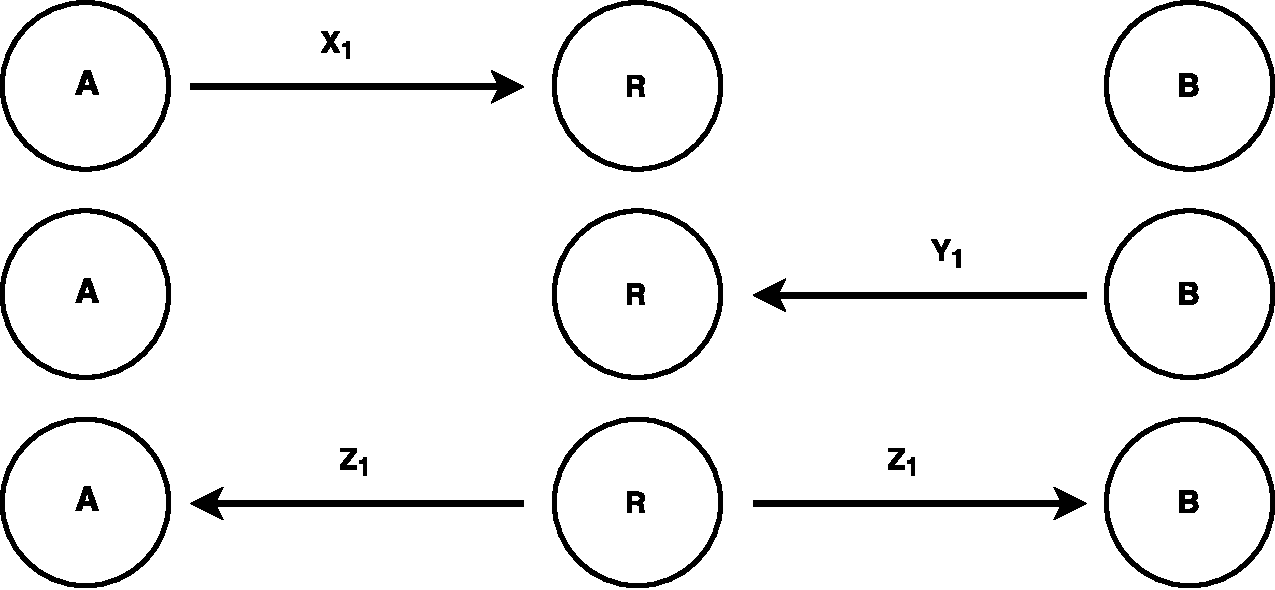
\includegraphics[width=0.8\textwidth]{figures/straightforwardNC.pdf}
    \caption{Straightforward network coding. First, $A$ transmits its packet to relay, then $B$ transmits its message to the relay, then relay calculates $Z_1=X_1 \oplus Y_1$ and broadcasts it to $A$ and $B$ in time slot three, which can then decode the other nodes message by another XOR.} \label{fig:straightforwardNC}
\end{figure}

\begin{figure} [th]
    \centering
    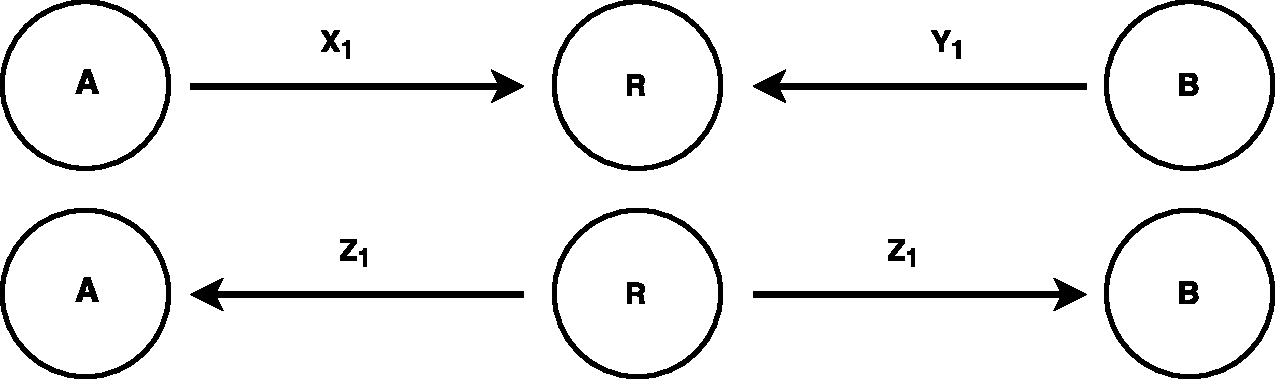
\includegraphics[width=0.8\textwidth]{figures/threeNodePnc.pdf}
    \caption{Physical layer network coding. In time slot one, $A$ and $B$ will transmit their packets to the relay at the same time (multiple access phase). The relay, using its mapping function extracts XOR of $A$ and $B$'s packets and broadcasts it to them in time slot two (broadcast phase).} \label{fig:threeNodePnc}
\end{figure}

Physical layer network coding is similar to straightforward networking coding with the difference that in PNC, the two messages from $A$ and $B$ are coded (combined) in the physical layer using the additive nature of simultaneously arriving electromagnetic (EM) waves \cite{zhang2006hot}. This reduces the number of time slots for the same exchange to happen to two. In a simple BPSK modulation where 0 and 1 are represented with $-1$ and $+1$ respectively, if $A$ and $B$ transmit their packet to the relay at the same time, they relay will received symbols of $-2$, $0$, and $+2$. At this step, every PNC capable relay requires a mapping function, to convert these new symbols into bits of data with a meaningful relationship to $A$ and $B$'s bits. In this simple BPSK example, mapping $-2$ and $+2$ symbols to 1 and $0$ symbols to 0, means that the received message at the relay is again XOR of $A$ and $B$'s packets. Just like the straightforward network coding, the relay then broadcasts this information back to $A$ and $B$ and they will use it to extract the other node's packet.

The same technique can be extended to linear multi-hop networks with more than two hops. Although a multi-hop scenario suffers from interference from other nodes, PNC is among technologies that can still maintain a reliable error rate and much higher throughput.


\section{Software Defined Radio}

\subsection{Overview}

Software Defined Radio (SDR) is a general term for describing a communication system where the main components are implemented in software instead of a hardware. Depending on the application, the software can be running on either a host computer or an embedded device. Developing radios in software has many advantages over hardware design. Software radio is a lot more rapid in development, it is easier to debug and it is customizable at a very low cost. Even in embedded system based SDR designs, the implementation can change with a new firmware, whereas a hardware system might need totally new device even for smallest modifications.

Fig. \ref{fig:sdr} shows main components of an SDR system. Analog to Digital Converter (ADC) and Digital to Analog Converter (DAC) are at the heart of every software defined radio. Since the carrier frequency for many protocols is much higher than hundreds of mega hertz, the signal received by the receiver chain antenna has a very high bandwidth which can not be directly converted to digital. Thus, a mixer would have to bring the received signal to baseband domain before being sampled by ADC. Similarly in the transmitter chain, the signal after DAC is in baseband and is brought to the required carrier frequency by an analog mixer.

\begin{figure} [th]
    \centering
    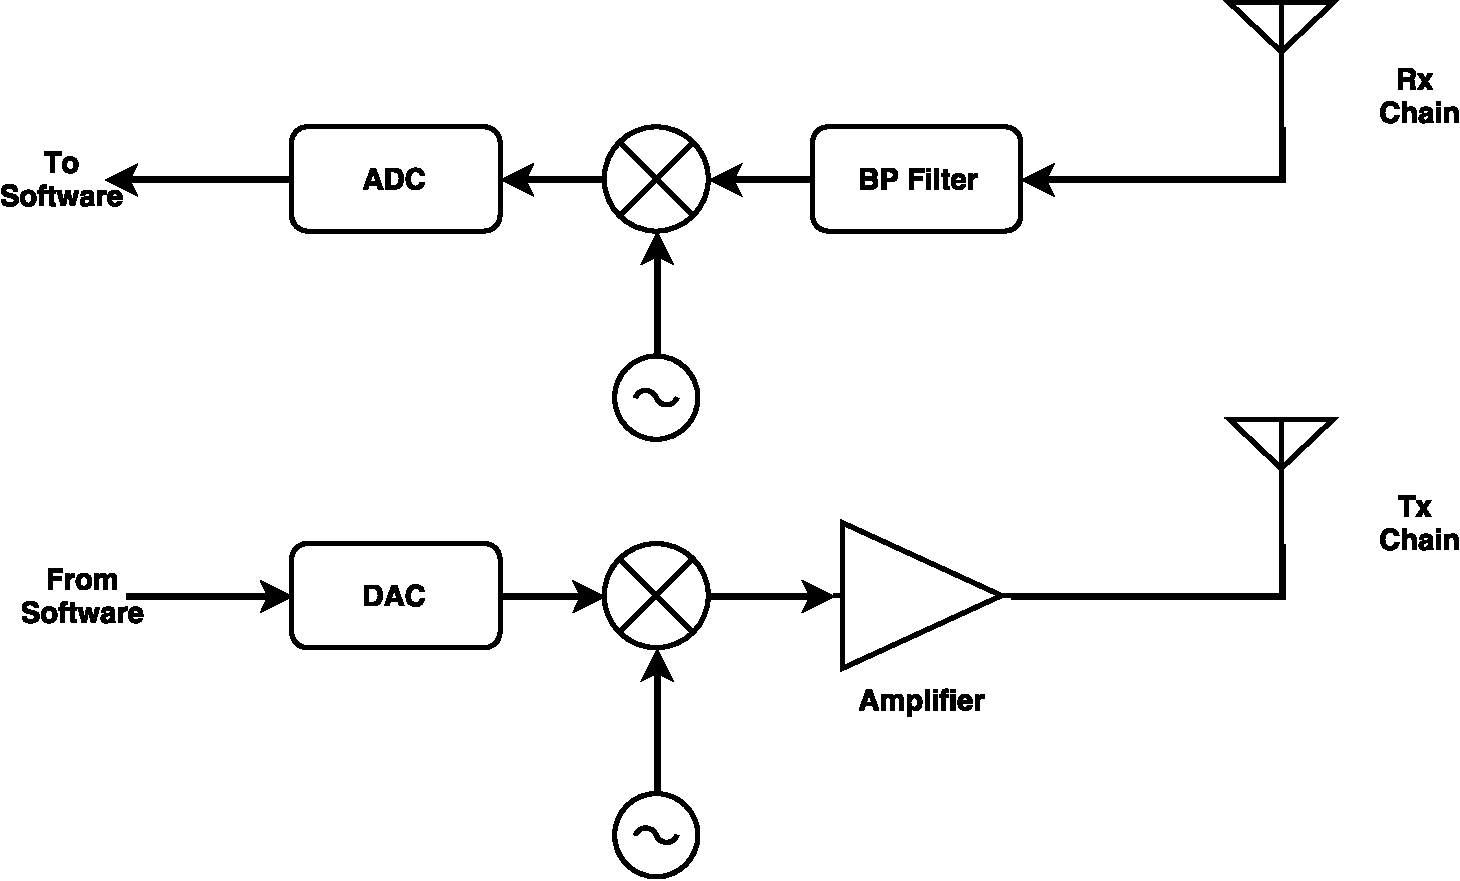
\includegraphics[width=0.8\textwidth]{figures/sdr.pdf}
    \caption{Simple illustration of software defined radio concept} \label{fig:sdr}
\end{figure}

\subsection{Universal Software Radio Peripheral}

Universal Software Radio Peripheral or USRP, is a famous SDR hardware by Ettus Research. USRPs have a motherboard with very accurate and high speed ADC and DAC, together with a Field-Programmable Gate Array (FPGA) for signal processing purposes. One of the key advantages of USRP is that it does the analog operations explained in the previous section on a different board than the motherboard. Daughterboards, as they are called by USRP community, have oscillators and mixers and analog amplifiers on them. Each daughterboard is designed for a specific range of frequency spectrum. This way, one can experiment on almost any frequency using the same motherboard by just using the appropriate daughterboard.

In normal applications, the FPGA on USRP adjusts the sampling rate of incoming and outgoing sample streams. Digital samples are transmitted to and received from a host computer using a LAN cable or USB. The FPGA is open to be programmed for high speed and low latency operations that can not tolerate the delay of communicating with a host computer.

USRP devices come with USRP Hardware Driver (UHD) to be installed on a normal computer. Using UHD, one can work with USRPs on MATLAB, Simulink, GNURadio or by writing softwares directly communicating with the UHD Application Programming Interface (API).


\subsection{GNURadio}

GNURadio is a free software by GNU project distributed under the terms of the GNU General Public License (GPL). It provides a software platform for signal processing and SDR systems. It can be used to either run pure simulations or interact with external hardware like USRP for SDR purposes. The user can implement arbitrary protocols by connecting different block and creating a flow graph for digital samples to be processed. GNURadio comes with many built-in blocks for modulation, coding, and many other signal processing functions. The user can also implement and add its own blocks to the platform. New blocks can be written in either C++ or Python language and blocks written in different languages can work together in the same system. This way, the user can have the advantages of Python and C++ together. Python can be use if rapid development is necessary and C++ language is used where optimization is concerned.